%auto-ignore
\begin{figure*}[ht!]
\begin{center}
\vspace{-10pt}
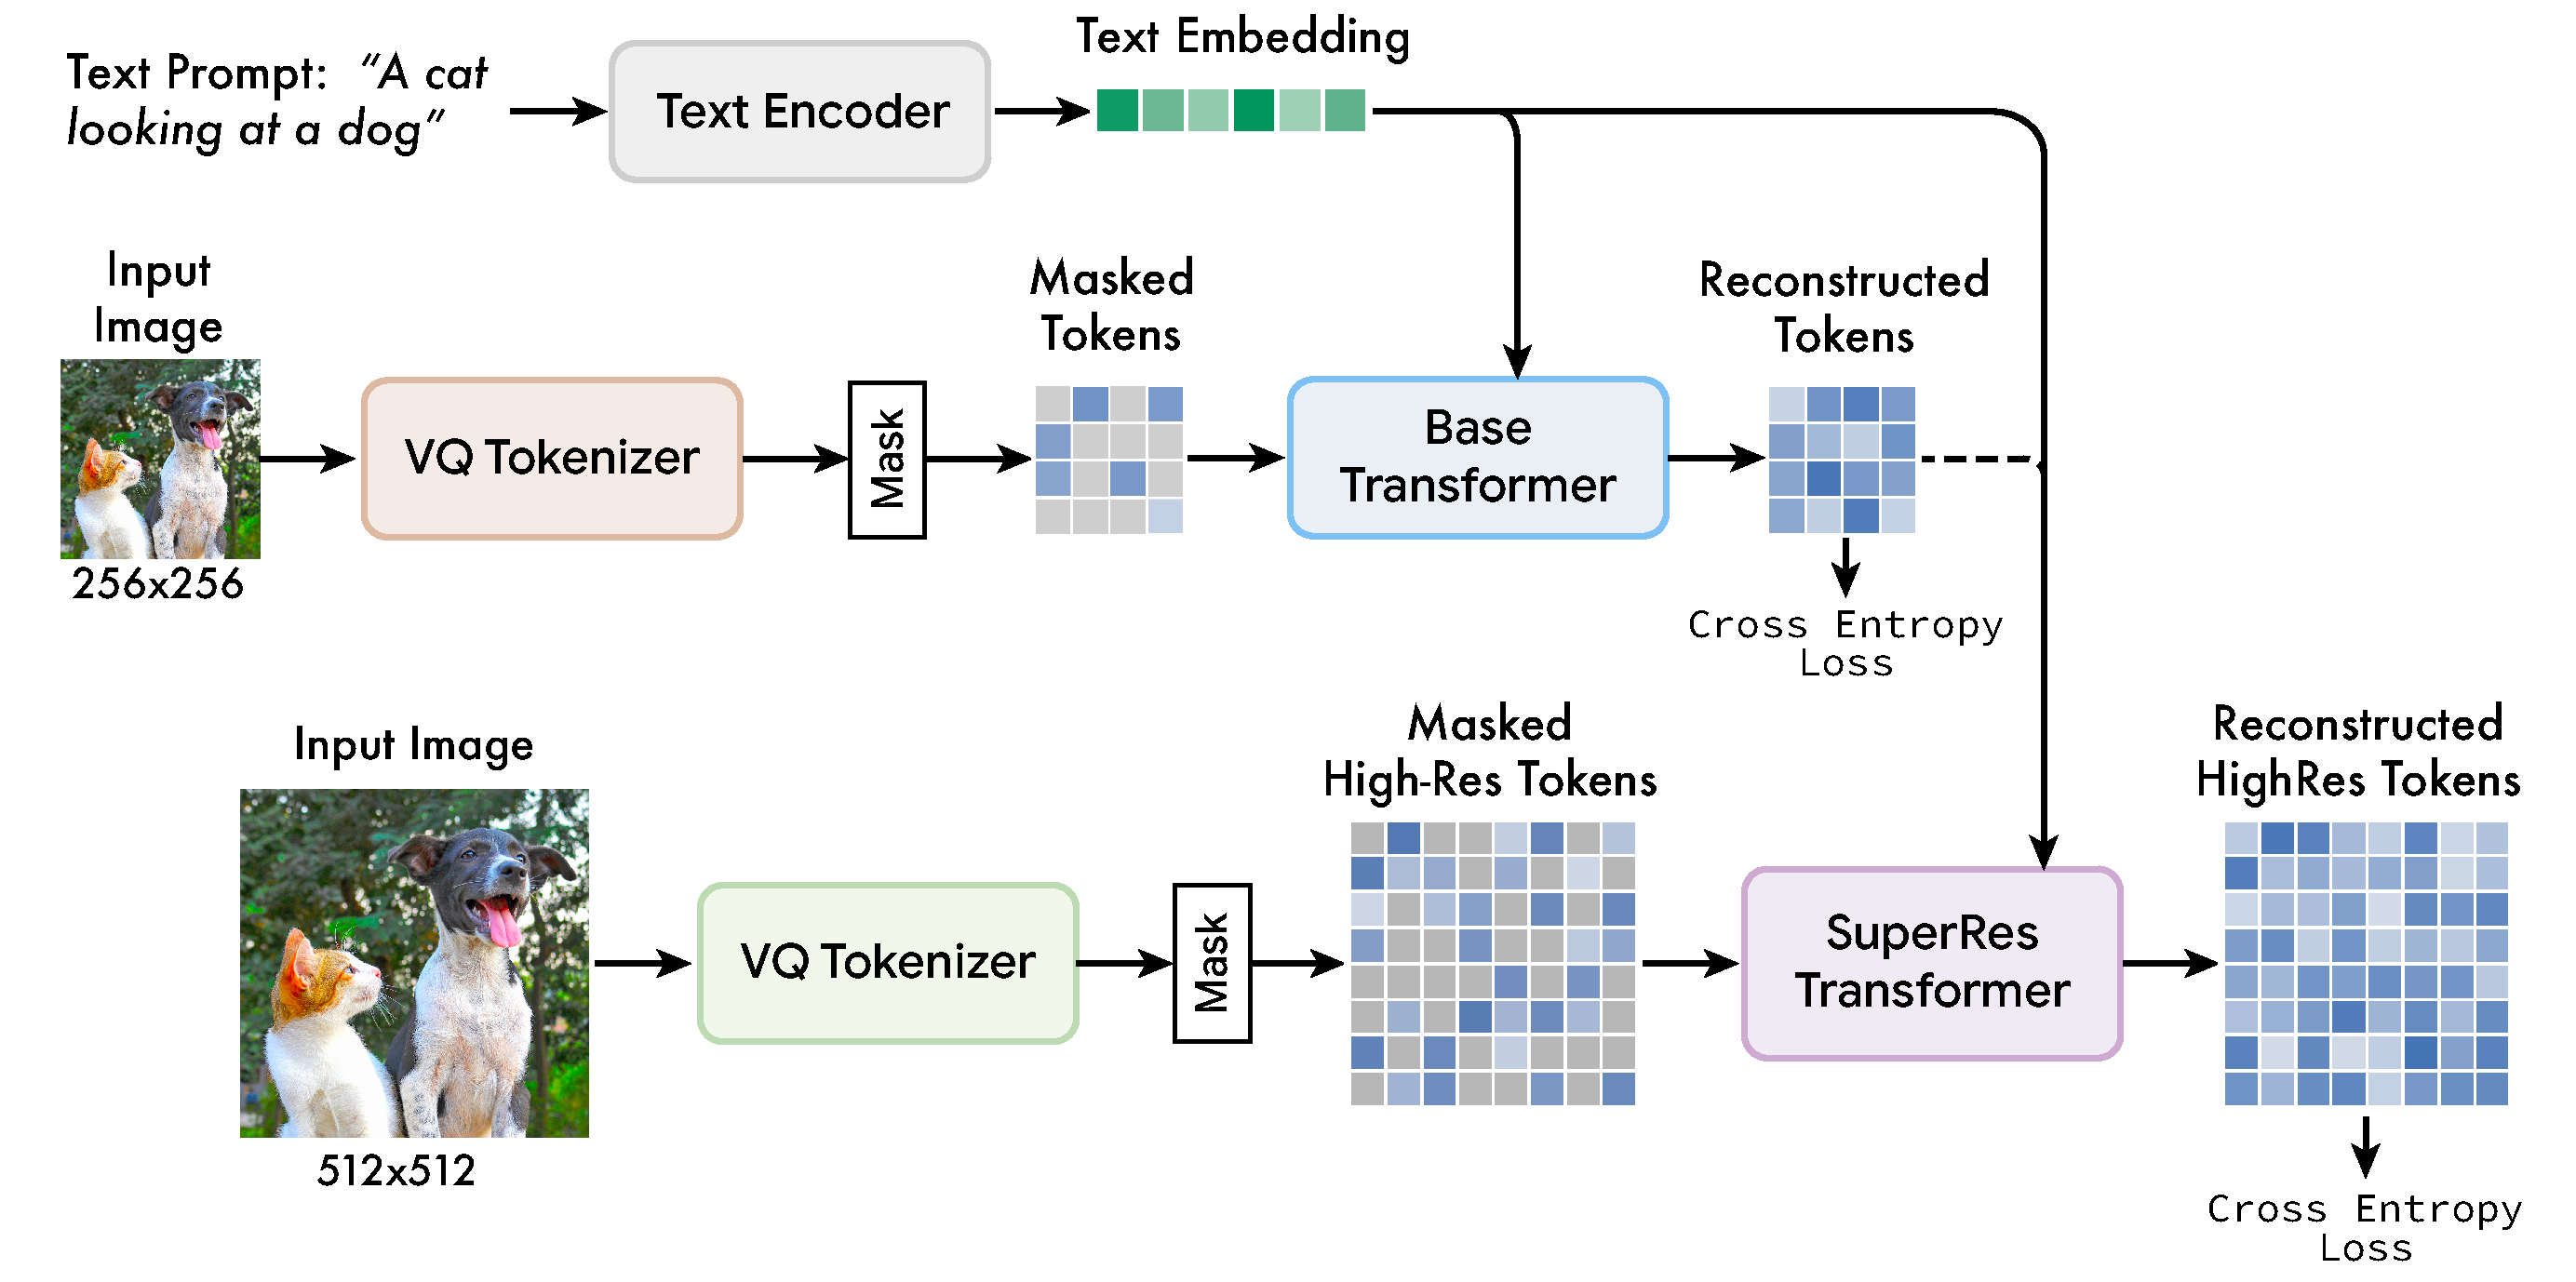
\includegraphics[width=.85\textwidth]{figs/pipeline_v4}
\end{center}
\vspace{-15pt}
\caption{\small \name~Framework: We show the training pipeline for our model, with the T5-XXL pre-trained text encoder, base model and super-resolution model depicted on the three rows. The text encoder generates a text embedding that is used for cross-attention with image tokens for both base and super-res Transformer layers. The base model uses a VQ Tokenizer that is pre-trained on lower resolution ($\lowres\times\lowres$) images and generates a $16\times16$ latent space of tokens. This sequence is masked at a variable rate per sample and then the cross-entropy loss learns to predict the masked image tokens. Once the base model is trained, the reconstructed lower-resolution tokens and text tokens are passed into the super-res model that then learns to predict masked tokens at a higher resolution. }

\vspace{-10pt}
\label{fig:model}
\end{figure*}

\section{Model}
\label{sec:model}
Our model is built on a number of components. Here, we provide an overview of each of those components in the order of their training, while relegating many details of the architecture and parameters to the Appendix. \figg{model} provides an overview of the model architecture. 

\subsection{Pre-trained Text Encoders}
Similar to the findings in \citep{imagen}, we find that leveraging a pre-trained large language model (LLM) is beneficial to high-quality image generation. The embeddings extracted from an LLM such as T5-XXL \citep{t5xxl} carry rich information about objects (nouns), actions (verbs), visual properties (adjectives), spatial relationships (prepositions), and other properties such as cardinality and composition. Our hypothesis is that the \name~model learns to map these rich visual and semantic concepts in the LLM embeddings to the generated images; it has been shown in recent work \citep{merullo2022linearly} that the conceptual representations learned by LLM's are roughly linearly mappable to those learned by models trained on vision tasks. Given an input text caption, we pass it through the frozen T5-XXL encoder, resulting in a sequence of 4096 dimensional language embedding vectors. These embedding vectors are linearly projected to the hidden size of our Transformer models (base and super-res).

\subsection{Semantic Tokenization using VQGAN}
\label{sec:vqgan}
A core component of our model is the use of semantic tokens obtained from a VQGAN \cite{esser2021taming} model. This model consists of an encoder and an decoder, with a quantization layer that maps an input image into a sequence of tokens from a learned codebook. We build our encoder and decoder entirely with convolutional layers to support encoding images from different resolutions. The encoder has several downsampling blocks to reduce the spatial dimension of the input, while the decoder has the corresponding number of upsampling blocks to map the latents back into original image size. Given an image of size $H \times W$, the encoded token is of size $\nicefrac{H}{f} \times \nicefrac{W}{f}$, with downsampling ratio $f$.
We train two VQGAN models: one with downsampling ratio $f=16$ and the other with downsampling ratio $f=8$. We obtain tokens for our base model using the $f=16$ VQGAN model on {\lowres}$\times${\lowres} pixel images, thus resulting in tokens with spatial size $16 \times 16$. We obtain the tokens for our super-resolution model using the $f=8$ VQGAN model on $512\times512$ images, and the corresponding token has spatial size $64\times64$. As mentioned in previous work \citep{esser2021taming}, the resulting discrete tokens after encoding capture higher-level semantics of the image, while ignoring low level noise. Furthermore, the discrete nature of these tokens allows us to use a cross-entropy loss at the output to predict masked tokens in the next stage.

%The resulting tokens capture higher-level semantics of the image, while ignoring low level noise. Furthermore, the discrete nature of these tokens allows us to use a cross-entropy loss at the output to predict masked tokens; and the resulting discrete probability distribution is used at inference time to enable parallel decoding. This approach follows that of MaskGit \citep{maskgit}, and makes our approach significantly more efficient than that of diffusion or autoregressive models. We train $2$ VQGAN models: one for the base model that works at $256\times256$ resolution and one for the super-resolution model that works at $512\times512$ resolution. For the first VQGAN, the latent space is a $16\times16$ map, i.e. the resulting token length if $256$. For the second VQGAN, the latent space is a $32\times32$ \aj{The superres section says that this is 64x64.} map (sequence length $1024$). \aj{Might be useful to point out that only the small encoder is used during based model training. And is the 256 decoder ever used again?} \han{Han/Huiwen: pls fix details here}.

\subsection{Base Model}

Our base model is a masked transformer\citep{vaswani2017attention,bert}, where the inputs are the projected T5 embeddings and image tokens. We leave all the text embeddings unmasked and randomly mask a varying fraction of image tokens  (see \secc{masking}) and replace them with a special \mask token \citep{maskgit}.
We then linearly map image tokens into image input embeddings of the required Transformer input/hidden size along with learned 2D positional embeddings. Following previous transformer architecture \citep{vaswani2017attention},  we use several transformer layers including self-attention block, cross-attention block and MLP block to extract features. At the output layer, an MLP is used to convert each masked image embedding to a set of logits (corresponding to the VQGAN codebook size) and a cross-entropy loss is applied with the ground truth token label as the target. At training, the base model is trained to predict all masked tokens at each step. However, for inference, mask prediction is performed in an iterative manner which significantly increases quality. See \secc{iterativedec} for details.
%\dilip{did we experiment with ablations such as self-attention on text tokens or dropping masked tokens from attention computation?} \huiwen{I think we have different text condition design ablations on small models without adafactor. Do you think it worths showing?} \dilip{yes - we can put it in the Appendix and refer to it here with a 1-sentence summary of the findings.}. At training, the base model chooses one random mask for each sample, and is trained to predict all masked tokens at each step. However, for inference, mask prediction is performed in an iterative manner which significantly increases quality. See \secc{iterativedec} for details.

\subsection{Super-Resolution Model}


\begin{figure*}[ht!]
\vspace{-10pt}
\begin{minipage}[c]{0.63\textwidth}
\centering
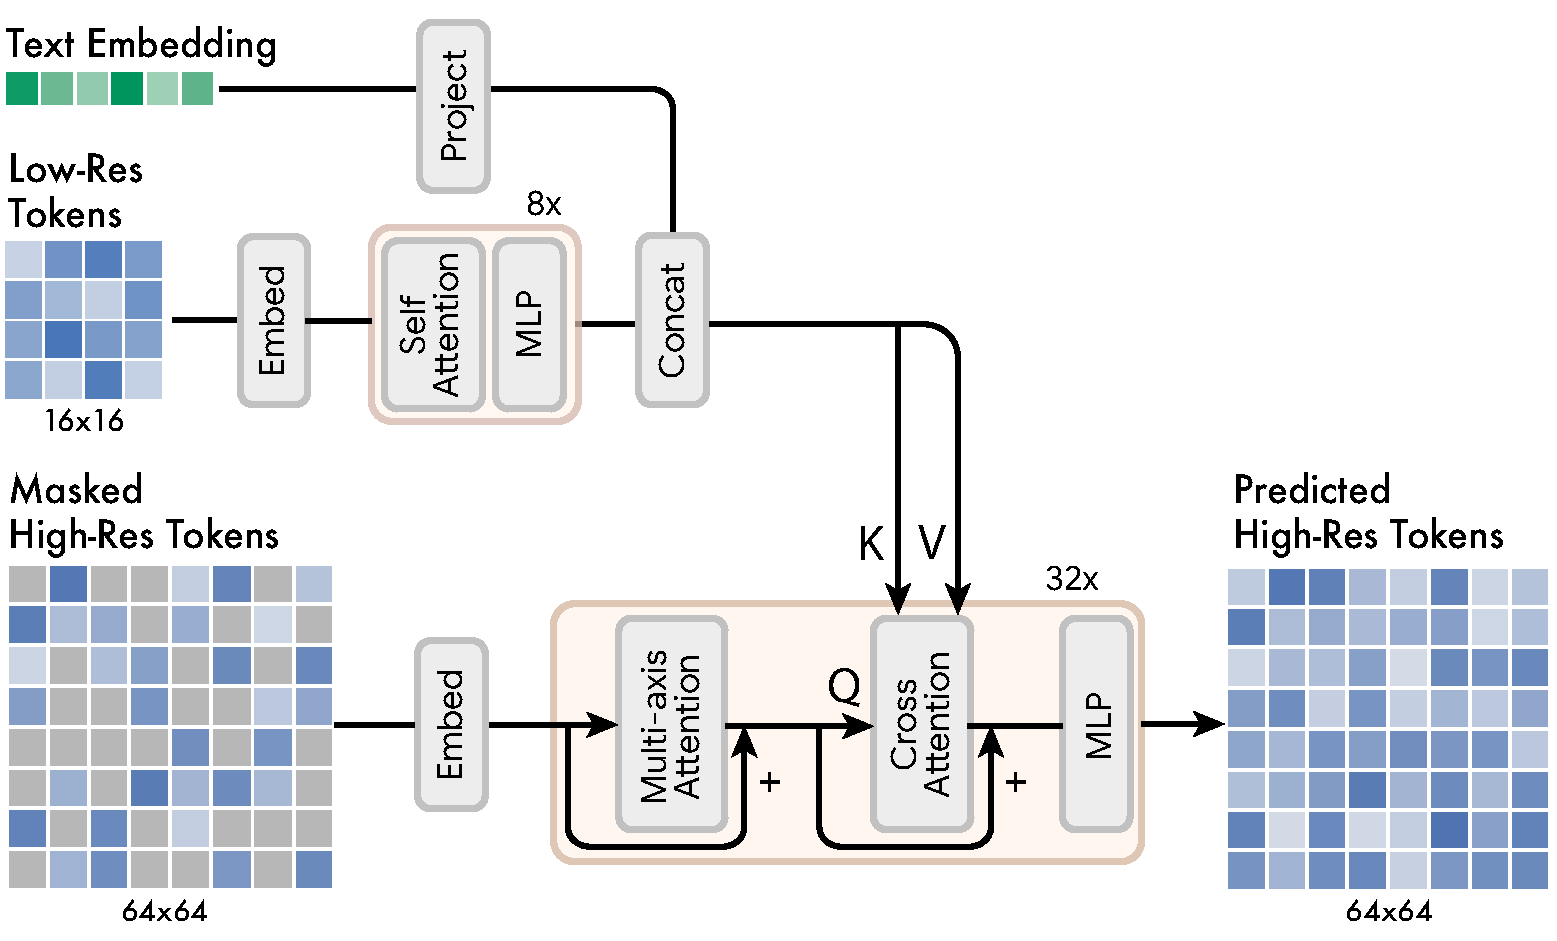
\includegraphics[width=\textwidth]{figs/superres_arch_fig}
%\caption{The architecture of the super-resolution model.}
\end{minipage} \hfill
%
\begin{minipage}[c]{0.34\textwidth}
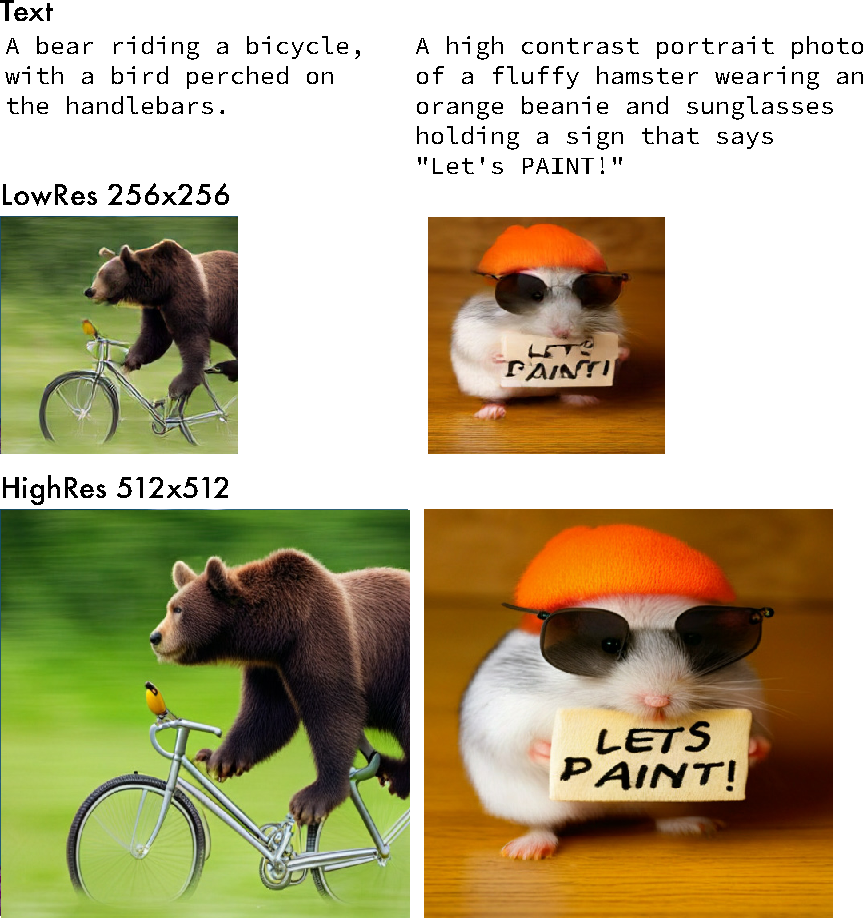
\includegraphics[width=\textwidth]{figs/superres_examples}
%\caption{Super-resolution examples.}
\end{minipage} 
\vspace{-5pt}
\caption{\small Super-resolution Model. On the left is shown the architecture of the super-resolution model. Low-resolution tokens are passed into a series of self-attention Transformer layers; and the resulting output embeddings are concatenated with text embeddings extracted from the conditioning text prompt. Following this, cross-attention is applied from these concatenated embeddings to the masked high-resolution tokens; the loss learns to predict these masked tokens conditioned on the low-resolution and text tokens. On the right are shown two examples of the improvement brought about by the super-resolution model.}

\label{fig:sr}
\end{figure*} 
We found that directly predicting $512\times512$ resolution leads the model to focus on low-level details over large-scale semantics. As a result we found it beneficial to use a cascade of models: first a base model that generates a $16\times16$ latent map (corresponding to a $\lowres \times \lowres$ image), followed by a super-resolution model that upsamples the base latent map to a $64\times64$ latent map (corresponding to a $512\times512$ image). The super-res model is trained after the base model has been trained.

As mentioned in \secc{vqgan}, we trained two VQGAN models, one at $16\times16$ latent resolution and $\lowres\times\lowres$ spatial resolution, and the second at $64\times64$ latent resolution and $512\times512$ spatial resolution. Since our base model outputs tokens corresponding to a $16\times16$ latent map, our super-resolution procedure learns to ``translate" the lower-resolution latent map to the higher-resolution latent map, followed by decoding through the higher-resolution VQGAN to give the final high-resolution image. This latent map translation model is also trained with text conditioning and cross-attention in an analogous manner to the base model, as shown in \figg{sr}. 

\subsection{Decoder Finetuning}
\label{sec:dec_finetune}
To further improve our model's ability to generate fine details, we increase the capacity of the VQGAN decoder by the addition of more residual layers and channels while keeping the encoder capacity fixed. We then finetune the new decoder layers while keeping the VQGAN encoder weights, codebook and transformers (i.e., base model and super resolution model) frozen. This allows us to improve our visual quality without re-training any of the other model components (because the visual token ``language'' stays fixed). This is shown in \figg{finetune_decoder} in the Appendix, where we see that the finetuned decoder can reconstruct more sharper details in the store front. We also give details of the finetuned decoder architecture in the Appendix.

\subsection{Variable Masking Rate}
\label{sec:masking}
As was done in \cite{maskgit}, we train our model with a variable masking rate based on a Cosine scheduling: for each training example, we sample a masking rate $r\in[0,1]$ from a truncated $\arccos$ distribution with density function $p(r)=\frac{2}{\pi}(1-r^2)^{-\frac{1}{2}}$. This has an expected masking rate of 0.64, with a strong bias towards higher masking rates. The bias towards higher masking rates makes the prediction problem harder. In contrast with autoregressive approaches, which learn conditional distributions $P(x_i | x_{<i})$ for some fixed ordering of tokens, random masking with a variable masking ratio allows our models to learn $P(x_i | x_{\Lambda})$ for arbitrary subsets of tokens $\Lambda$. This is not only critical for our parallel sampling scheme, but it also enables a number of zero-shot, out-of-the-box editing capabilities, such as shown in \figg{teaser_edit} and \secc{editing}.

\subsection{Classifier Free Guidance}
\label{sec:cfg}
We employ classifier-free guidance (CFG) \citep{ho2022classifier} to improve our generation quality and our text-image alignment. At training time, we remove text conditioning on 10\% of samples chosen randomly (thus attention reduces to image token self-attention). At inference time, we compute a conditional logit $\ell_c$ and an unconditional logit $\ell_u$ for each masked token. We then form the final logits $\ell_g$ by moving away from the unconditional logits by an amount $t$, the \emph{guidance scale}:
\begin{equation}
    \ell_g = (1+t)\ell_c - t \ell_u
    \label{eq:cfg}
\end{equation}
Intuitively, CFG trades off diversity for fidelity. Different from previous approaches, we reduce the hit to diversity by linearly increasing the guidance scale $t$ through the sampling procedure. This allows the early tokens to be sampled more freely, with low or no guidance, but increases the influence of the conditioning prompt for the later tokens.

We also exploit this mechanism to enable \emph{negative prompting} \citep{negprompt} by replacing the unconditional logit $\ell_u$ with a logit conditioned on a ``negative prompt''. This encourages the resulting image to have features associated with the positive prompt $\ell_c$ and remove features associated with the negative prompt $\ell_u$. 
%We found this to be particularly useful for reducing the effects of watermarked images in the training set.
\subsection{Iterative Parallel Decoding at Inference}
\label{sec:iterativedec}
\begin{figure*}[ht!]
\begin{center}
\vspace{-5pt}
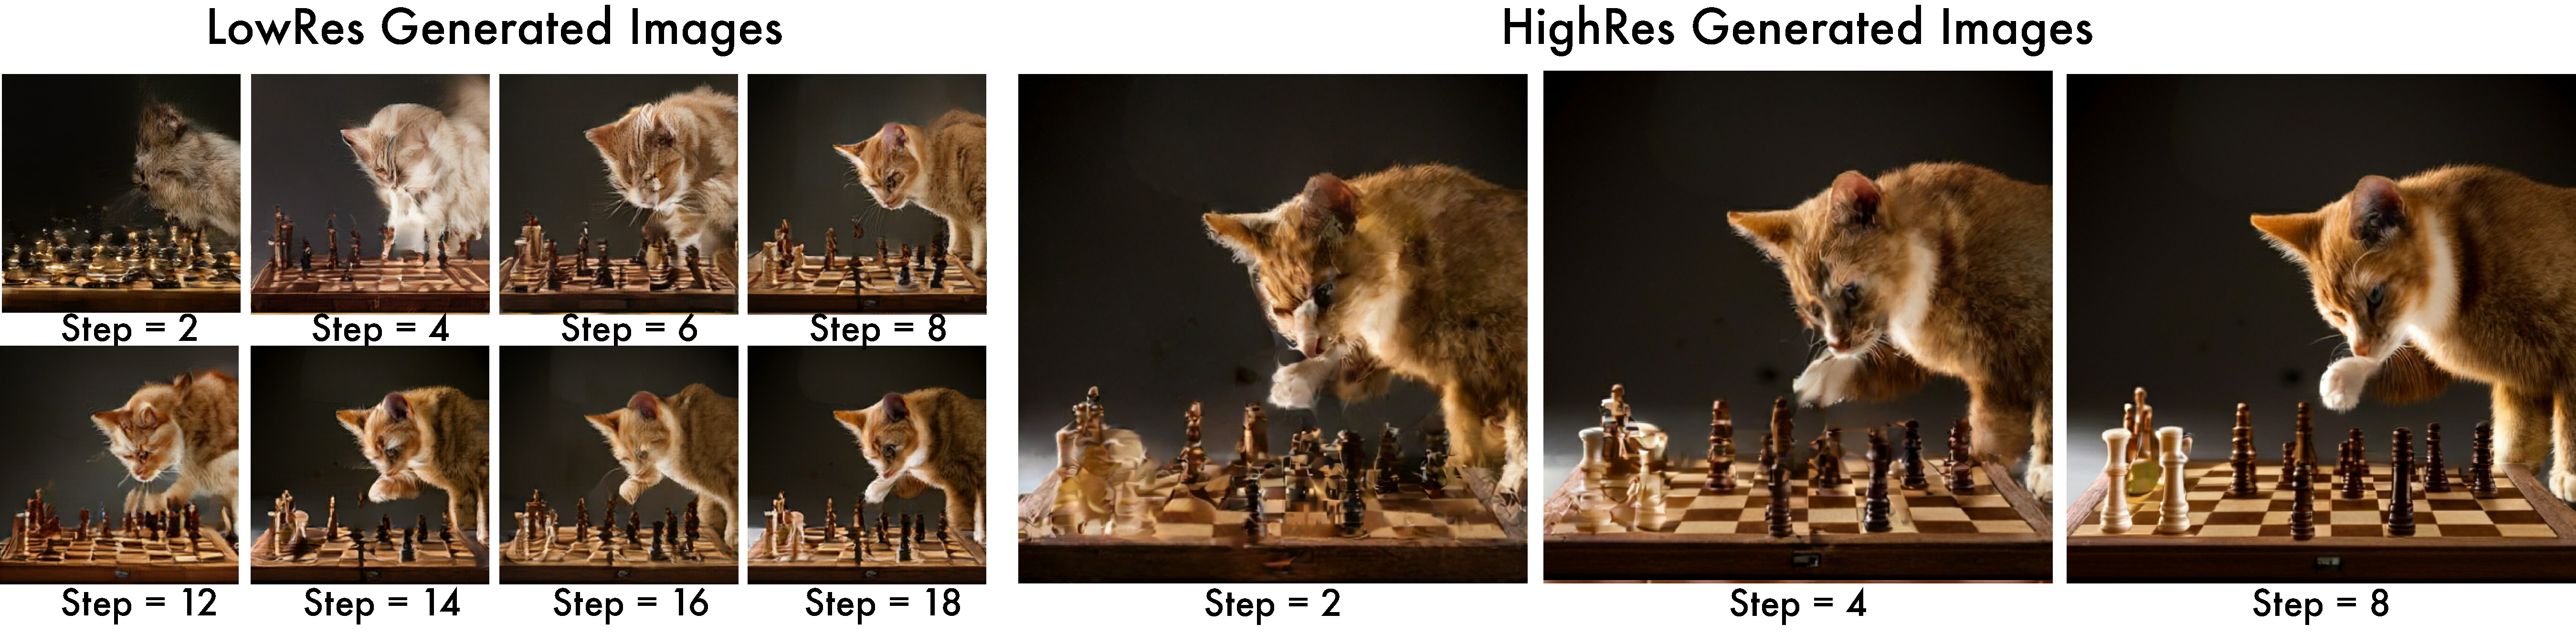
\includegraphics[width=1.0\textwidth]{figs/inference_fig}
\end{center}
\vspace{-10pt}
\caption{\small Inference samples. We visualize the evolution of masked tokens over the sequence of steps for the base model (left) and the super-res model (right). The super-res model, being conditioned on the low-res tokens, requires significantly fewer sampling steps for convergence. 
% \huiwen{this is a placeholder, will add text prompt and maybe change the image to something that is not with white background \dilip{is this still a placeholder? Looks good to me}.}
}
\vspace{-5pt}
\label{fig:srmodel}
\end{figure*}
The critical component for our model's inference time efficiency is the use of parallel decoding to predict multiple output tokens in a single forward pass. The key assumption underlying the effectiveness of the parallel decoding is a Markovian property that many tokens are conditionally independent given other tokens. Decoding is performed based on a cosine schedule \citep{maskgit} that chooses a certain fixed fraction of the highest confidence masked tokens that are to be predicted at that step. These tokens are then set to unmasked for the remainder of the steps and the set of masked tokens is appropriately reduced. Using this procedure, we are able to perform inference of $256$ tokens using only $24$ decoding steps in our base model and $4096$ tokens using $8$ decoding steps in our super-resolution model, as compared to the 256 or 4096 steps required for autoregressive models (e.g. \citep{parti}) and hundreds of steps for diffusion models (e.g., \citep{ldm,imagen}). We note that recent methods including progressive distillation \citep{salimans2022distillation} and better ODE solvers \citep{Zhu2022dpm} have greatly reduced the sampling steps of diffusion models, but they have not been widely validated in large scale text-to-image generation. We leave the comparison to these faster methods in the future work, while noting that similar distillation approaches are also a possibility for our model.
